\vspace{10pt}

{\centering\subsection*{徐诗言:我的乐园}}

\addcontentsline{toc}{subsection}{徐诗言:我的乐园}

\renewcommand{\leftmark}{徐诗言:我的乐园}

\begin{figure}[htbp]

\centering

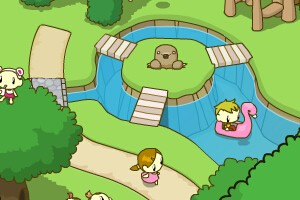
\includegraphics[width = .5\textwidth]{./ch/32.jpg}

\end{figure}



不论是谁,都会有自己的乐园,而我的乐园是公园的草坪。



一天,我和几个小妹妹还有爸爸妈妈们一起到公园去玩。其中一个妹妹,骑了一辆粉色的自行车,另外两个妹妹拿上了一根皮筋,过了一会儿,我们到了公园。



公园里有许许多多的人,简直是人山人海,我们来到草地上,爸爸和妈妈去散步、运动。一个妹妹去骑自行车,而我和另外两个妹妹一起跳皮筋,那个草地上有花儿、蝴蝶和小蚂蚁……那里的人们有的散步、玩游戏、跑步……



我们玩了一会儿,我和骑自行车的那个妹妹换了一下,我去骑自行车,很快我就追上了爸爸妈妈。又过了十几分钟,我们集体躺在草地上,仰起脸望向天空,这时天空非常的蓝,我看见天上的白云,有的像金鱼,有的像龙虾,有的像马儿,还有的像美人鱼,这些云彩可真奇幻啊!



大家一起在公园里愉悦的玩耍,多么开心,多么快乐呀!





\vspace{10pt}



作者:四(2)班 徐诗言



指导老师:陈小丽



投稿:2021年4月27日





发表:2021年4月30日






                



\vspace{10pt}

\hline



